\documentclass[article, 1.5space, letterpaper, 12pt, oneside, header, footer]{SydeClass}
\graphicspath{{images/}}
\usepackage{subfigure}
\usepackage{eqnarray}


% --------- Title Info -----------
\titlestyle{design} % used in SydeTitle.tex. Can equal one of the following values: design, work

\title{Lab 1}
\subtitle{Fundamentals of Image Processing}

\coursecode{SYDE 475}
\department{Systems Design Engineering}

\author{Colin Heics, 20240543}
\authorheader{C. Heics}
\authortwo{Neil Sokol, 20265064}
\authorheadertwo{N. Sokol}

\date{\today}
\instructor{Alex Wong}

\subsectionfont{\normalsize}
\setcounter{secnumdepth}{2}
\setcounter{tocdepth}{1}

\usepackage{listings}
\usepackage{color}
\usepackage{textcomp}
\definecolor{listinggray}{gray}{0.9}
\definecolor{lbcolor}{rgb}{0.9,0.9,0.9}
\lstset{
	backgroundcolor=\color{lbcolor},
	tabsize=4,
	rulecolor=,
	language=matlab,
        basicstyle=\scriptsize,
        upquote=true,
        aboveskip={1.5\baselineskip},
        columns=fixed,
        showstringspaces=false,
        extendedchars=true,
        breaklines=true,
        prebreak = \raisebox{0ex}[0ex][0ex]{\ensuremath{\hookleftarrow}},
        frame=single,
        showtabs=false,
        showspaces=false,
        showstringspaces=false,
        identifierstyle=\ttfamily,
        keywordstyle=\color[rgb]{0,0,1},
        commentstyle=\color[rgb]{0.133,0.545,0.133},
        stringstyle=\color[rgb]{0.627,0.126,0.941},
}

% ############  ############
\begin{document}

% ---------- Title ------------

%% Use the command "
%% Use the command "
%% Use the command "\input{SydeTitle}" in your main file to include this file.

\begin{titlepage}
	\makeatletter % use .cls usage for <at>
	
	\pagestyle{empty}
	\equalmargins
	
	\ifthenelse{\equal{\@titlestyle}{work}}{
		\begin{center}
			\vspace*{2em}

			University of Waterloo\\
			Faculty of Engineering\\
			Department of Systems Design Engineering

			\null\vfill
		
			\Huge\@title \\
			\ifdefined \@subtitle \Large\@subtitle \\ \fi
			\normalsize

			\null\vfill
		
			\@company\\
			\@companyaddress \vspace{2em}
		
			\@author\\
			\@date
		\end{center}
	}{\relax} % end if
	
	\ifthenelse{\equal{\@titlestyle}{design}}{
		\begin{center}
			\vspace*{5em}
	
			\Huge\@title \\
			\ifdefined \@subtitle \Large\@subtitle \\ \fi
			\normalsize
	
			\vfill
		
			A Report Submitted in Partial Fulfilment\\
			of the Requirements for \@coursecode \vspace{4em}
		
			\ifdefined \@groupname \@groupname \\ \fi
		  \@author \\
			\ifdefined \@authortwo \@authortwo \\ \fi
			\ifdefined \@authorthree \@authorthree \\ \fi
			\ifdefined \@authorfour \@authorfour \\ \fi
		  \vspace{3em}
		
			Faculty of Engineering \\
			\ifdefined \@department Department of \@department \\ \fi
			\vspace{3em}
		
			\@date \\
			
			\ifdefined \@instructor Course Instructor: \@instructor \\ \fi
			\ifdefined \@supervisor Project Supervisor: \@supervisor \\ \fi
			
		\end{center}
	}{\relax} % end if
	
	\makeatother % return to document usage for <at>
\end{titlepage}

%\pagestyle{plain}
%\offsetmargins" in your main file to include this file.

\begin{titlepage}
	\makeatletter % use .cls usage for <at>
	
	\pagestyle{empty}
	\equalmargins
	
	\ifthenelse{\equal{\@titlestyle}{work}}{
		\begin{center}
			\vspace*{2em}

			University of Waterloo\\
			Faculty of Engineering\\
			Department of Systems Design Engineering

			\null\vfill
		
			\Huge\@title \\
			\ifdefined \@subtitle \Large\@subtitle \\ \fi
			\normalsize

			\null\vfill
		
			\@company\\
			\@companyaddress \vspace{2em}
		
			\@author\\
			\@date
		\end{center}
	}{\relax} % end if
	
	\ifthenelse{\equal{\@titlestyle}{design}}{
		\begin{center}
			\vspace*{5em}
	
			\Huge\@title \\
			\ifdefined \@subtitle \Large\@subtitle \\ \fi
			\normalsize
	
			\vfill
		
			A Report Submitted in Partial Fulfilment\\
			of the Requirements for \@coursecode \vspace{4em}
		
			\ifdefined \@groupname \@groupname \\ \fi
		  \@author \\
			\ifdefined \@authortwo \@authortwo \\ \fi
			\ifdefined \@authorthree \@authorthree \\ \fi
			\ifdefined \@authorfour \@authorfour \\ \fi
		  \vspace{3em}
		
			Faculty of Engineering \\
			\ifdefined \@department Department of \@department \\ \fi
			\vspace{3em}
		
			\@date \\
			
			\ifdefined \@instructor Course Instructor: \@instructor \\ \fi
			\ifdefined \@supervisor Project Supervisor: \@supervisor \\ \fi
			
		\end{center}
	}{\relax} % end if
	
	\makeatother % return to document usage for <at>
\end{titlepage}

%\pagestyle{plain}
%\offsetmargins" in your main file to include this file.

\begin{titlepage}
	\makeatletter % use .cls usage for <at>
	
	\pagestyle{empty}
	\equalmargins
	
	\ifthenelse{\equal{\@titlestyle}{work}}{
		\begin{center}
			\vspace*{2em}

			University of Waterloo\\
			Faculty of Engineering\\
			Department of Systems Design Engineering

			\null\vfill
		
			\Huge\@title \\
			\ifdefined \@subtitle \Large\@subtitle \\ \fi
			\normalsize

			\null\vfill
		
			\@company\\
			\@companyaddress \vspace{2em}
		
			\@author\\
			\@date
		\end{center}
	}{\relax} % end if
	
	\ifthenelse{\equal{\@titlestyle}{design}}{
		\begin{center}
			\vspace*{5em}
	
			\Huge\@title \\
			\ifdefined \@subtitle \Large\@subtitle \\ \fi
			\normalsize
	
			\vfill
		
			A Report Submitted in Partial Fulfilment\\
			of the Requirements for \@coursecode \vspace{4em}
		
			\ifdefined \@groupname \@groupname \\ \fi
		  \@author \\
			\ifdefined \@authortwo \@authortwo \\ \fi
			\ifdefined \@authorthree \@authorthree \\ \fi
			\ifdefined \@authorfour \@authorfour \\ \fi
		  \vspace{3em}
		
			Faculty of Engineering \\
			\ifdefined \@department Department of \@department \\ \fi
			\vspace{3em}
		
			\@date \\
			
			\ifdefined \@instructor Course Instructor: \@instructor \\ \fi
			\ifdefined \@supervisor Project Supervisor: \@supervisor \\ \fi
			
		\end{center}
	}{\relax} % end if
	
	\makeatother % return to document usage for <at>
\end{titlepage}

%\pagestyle{plain}
%\offsetmargins

% ############ Chapters ############
\pagenumbering{arabic}

\section{Introduction}



\section{Image quality measures}

During the lab, some operations will be applied to a modified image in order to imporve it's appearance. In order to evaluate the quality of the operation, a measure known as the ``Peak Signal to Noise Ratio'' (PSNR) is used, calculated as illustrated in \eqref{eqn-psnr}.

\begin{eqnarray}
\label{eqn-psnr}
PSNR & = & 10 \log_{10}\left ( \frac{{\textup{MAX}_f}^{2}}{\textup{MSE}} \right ) \\
\textup{MSE} & = &\frac{1}{mn} \sum_{i=0}^{m-1}\sum_{j=0}^{n-1} \left \| f(i,j) - g(i,j) \right \|^2
\end{eqnarray}

The Matlab code used to calculate the PSNR for this lab is attached in Appendix~\ref{code-PSNR}.


\section{Digital zooming}

Digital zooming techniques can introduce artifacts into an image. In order to evaluate several digital zooming techniques, two different sample images will be douwn scaled by a factor of 4, then enlarged using one of three digital zooming techniques. The resulting images will be compared to the ground truth using PSNR, and are included in Figures~\ref{fig:digitalZoom.lena}~and~\ref{fig:digitalZoom.cameraman}.


\begin{figure}[ht]
\centering
	\subfigure[Original image, PSNR $= \infty$]{
	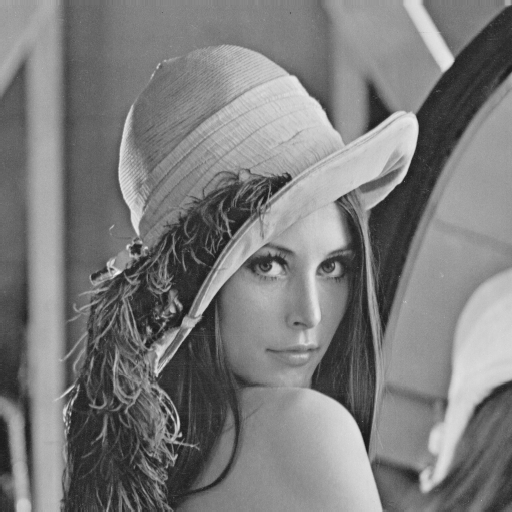
\includegraphics[width=0.45\linewidth]{digitalZoom/lenaBase}
	}
	\subfigure[Nearest Neighbor, PSNR = +33.96 dB]{
	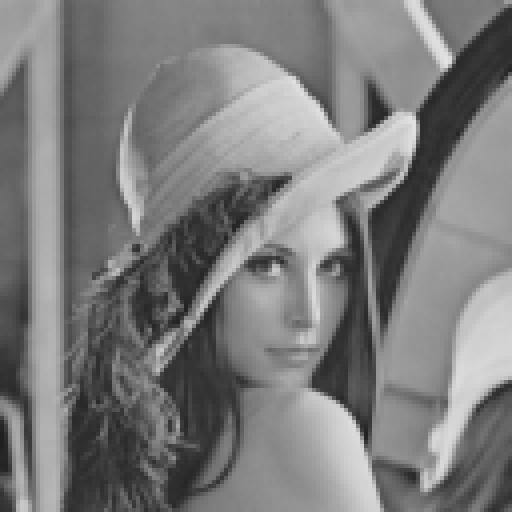
\includegraphics[width=0.45\linewidth]{digitalZoom/lena_NN}
	}
	\subfigure[Bilinear Interpolation, PSNR = +34.26 dB]{
	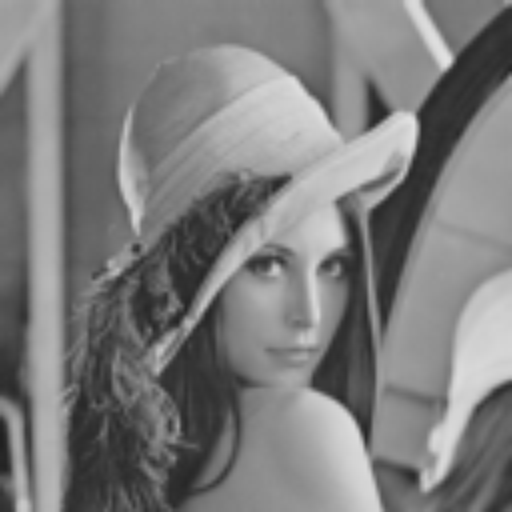
\includegraphics[width=0.45\linewidth]{digitalZoom/lena_BL}
	}
	\subfigure[Bicubic Interpolation, PSNR = +34.70 dB]{
	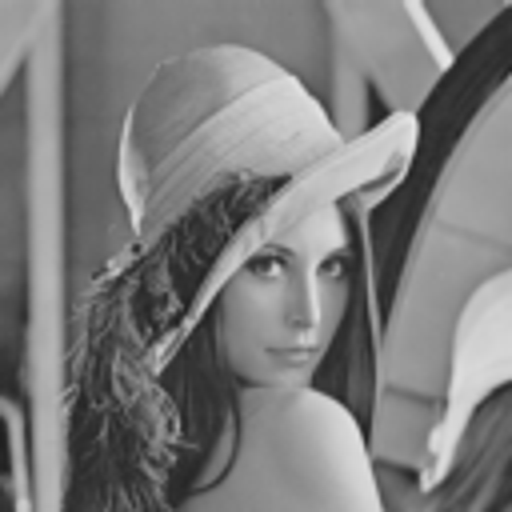
\includegraphics[width=0.45\linewidth]{digitalZoom/lena_BC}
	}
	\caption{Various methods of digitally zooming the Lena test image.}
	\label{fig:digitalZoom.lena}
\end{figure}

\begin{figure}[ht]

\centering
	\subfigure[Original image, PSNR $= \infty$]{
	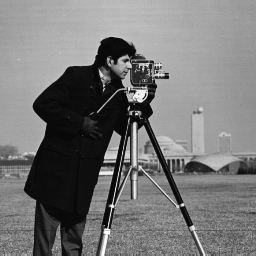
\includegraphics[width=0.45\linewidth]{digitalZoom/cameramanBase}
	}
	\subfigure[Nearest Neighbor, PSNR = +32.91 dB]{
	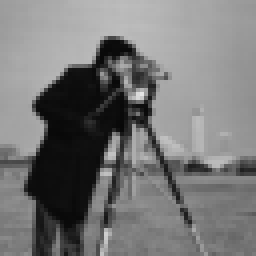
\includegraphics[width=0.45\linewidth]{digitalZoom/cameraman_NN}
	}
	\subfigure[Bilinear Interpolation, PSNR = +32.62 dB]{
	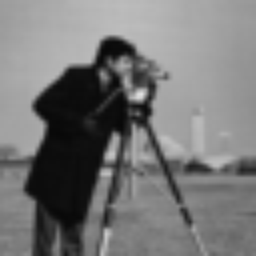
\includegraphics[width=0.45\linewidth]{digitalZoom/cameraman_BL}
	}
	\subfigure[Bicubic Interpolation, PSNR = +32.88 dB]{
	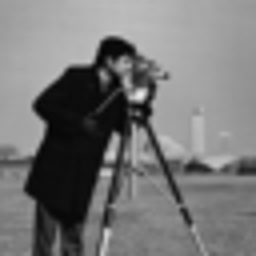
\includegraphics[width=0.45\linewidth]{digitalZoom/cameraman_BC}
	}
	\caption{Various methods of digitally zooming the Cameraman test image.}
	\label{fig:digitalZoom.cameraman}
\end{figure}

Note that since Matlab already has image resizing functions providing the various digital zooming techniques compared, and the lab instructions have not explicitly asked for a implementation, the Matlab function \texttt{imresize} is used.



\subsection{Discussion questions}

\subsubsection{What can you observed about the up-sampled images produced by each of the methods?}

Taking a look at the upsampled images in Figures~\ref{fig:digitalZoom.lena}~and~\ref{fig:digitalZoom.cameraman} we can qualitatively observe that the images look different.

The \emph{Nearest Neighbor} digital zooming approach has a blocky look (zooming the PDF or viewing a hardcopy is nessecary due to the limited PPI of LCD displays). This gives a blocky look to the image, as the algorithim is replacing each 1 pixel in the reduced size image with 16 of the same colour.

The \emph{Bilinear Interpolation} digital zooming approach has a blurred appearance. Bilinear interpolation interpolates using a quadratic polynomial (2 linear loopups); which smooths out the transitions between pixels. In low frequency detail regions, the transition looses the blocky look of the nearest neighbor zooming technique, but in high frequency areas the image loops blurry.

The \emph{Bicubic Interpolation} digital zooming approach has the best subjective appearance. Bicubic interpolation uses 16 pixels in order to derive the polynomial to lookup the new pixel values. Using a higher order polynomial allows detail to be better preserved in high frequency detail areas.

\subsubsection{How do the different methods compare to each other in terms of PSNR as well as visual quality? Why?}

As higher order digital zooming methods are used, the PSNR increases. Information is lost when the image is downsampled by a factor of 4 using the 1st order image resizing method. The higher order up-sampling methods are better at reconstructing high frequency detail from the downsampled image and therefore appear less fuzzy than the lower order methods. The higher order methods are also better at preserving edge contrast, which increases the percieved sharpness of the image; therefore the image looks ``better''.

\subsubsection{What parts of the image seems to work well using these digital zooming methods? What parts of the
image doesn't? Why?}

In large solid colour areas, all of the digital zooming methods perform equally. Lena's right shoulder is an area containing low frequency detail that looks very similar among all methods.

Low frequency gradations in the images look better using bilinear and bicubic, as interpolation allows for smooth transition between pixels. This is visible in the shading on Lena's face and the background of the Cameraman photo.

Image edges loose the staircase effect due to interpolation reducing edge aliasing. The edges of the photographer in the Cameraman photo look much better in the bilinear and bicubic photos.


High frequency details, such as Lena's eyes and the feathers in Lena's hat, look better in the bicubic and nearest neighbor digital zooms. The bilinear approach oversmooths the features of the images, and the detail contrast is reduced. The higher order interpolation is able to better interpolate the high frequency data and represent the eyes and feathers accurately.


\subsubsection{Compare the zooming results between Lena and Cameraman. Which image results in higher PSNR? Why?}

The digital zooms of Lena have higher PSNR for all digital zooming methods. This is because the Lena image has less high frequency components than the Cameraman image. Since all interpolation methods work more poorly with the high frequency areas of the image, an image that is composed of more high frequency components will look worse than one with fewer when zoomed using interpolation.


\subsubsection{Which image looks better when restored to the original resolution using digital zooming methods?}

Subjectively (and objectively according the to the PSNR measure), the Lena image looks closer to the original when zoomed using all digital zooming methods.


\subsubsection{What does the PSNR tell you about each of the methods? Does it reflect what is observed visually?}

Since PSNR quantifies the error in the image from the ground truth image, it illustrates that the two images compared using the PSNR measure are similar in intensity at the same points.

The images with higher PSNR generally look subjectively better. The exception is that the nearest neighbor Lena image looks better than bilinear Lena due to the bluriness induce by the bilinear interpolation. There exist other more complicated methods such as the Structural Similarity Method \cite{ssim-image-qual} and the Universal Image Quality Assesment Method \cite{universal-image-qual} (among many others) which may come to the same conclusion that I did about the images, as PSNR does not take into account the psychovisual model of human vision.


\clearpage
\section{Discrete convolution for image proccessing}



\begin{figure}[ht]
\centering
	\subfigure[Original image]{
	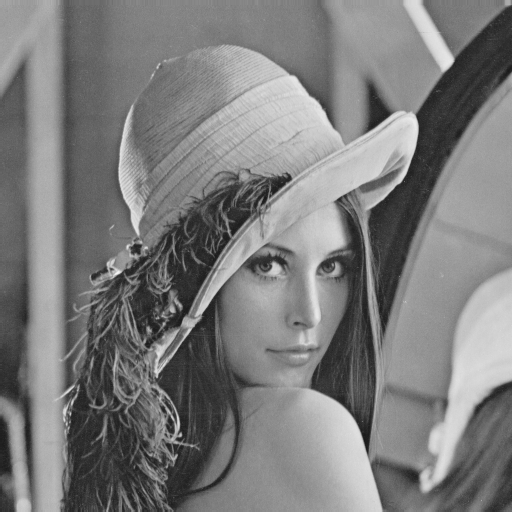
\includegraphics[width=0.45\linewidth]{discreteConvolution/lenaBase}
	}
	\subfigure[(0.16, 0.16, 0.16, 0.16, 0.16, 0.16) kernel]{
	%\caption{Convolved with $\left [ 0.16, 0.16, 0.16, 0.16, 0.16, 0.16\right ]$}
	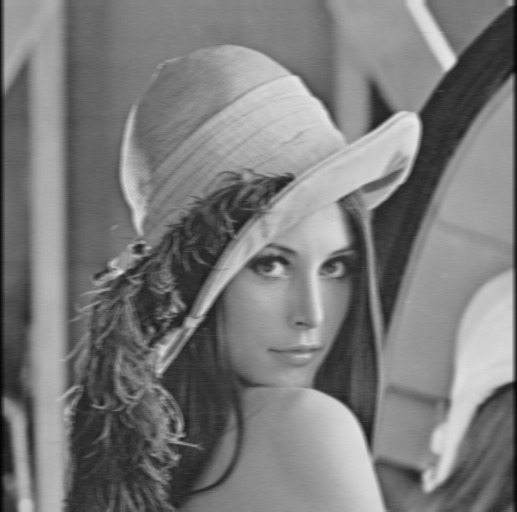
\includegraphics[width=0.45\linewidth]{discreteConvolution/lena_h1}
	}
	\subfigure[(0.16, 0.16, 0.16, 0.16, 0.16, 0.16)$^T$ kernel]{
	%\caption{Convolved with $\left [0.16, 0.16, 0.16, 0.16, 0.16, 0.16\right ]^\textup{T}$}
	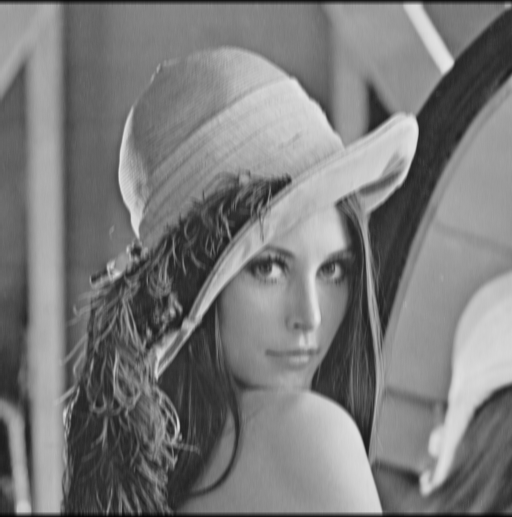
\includegraphics[width=0.45\linewidth]{discreteConvolution/lena_h2}
	}
	\subfigure[(1, -1) kernel]{
	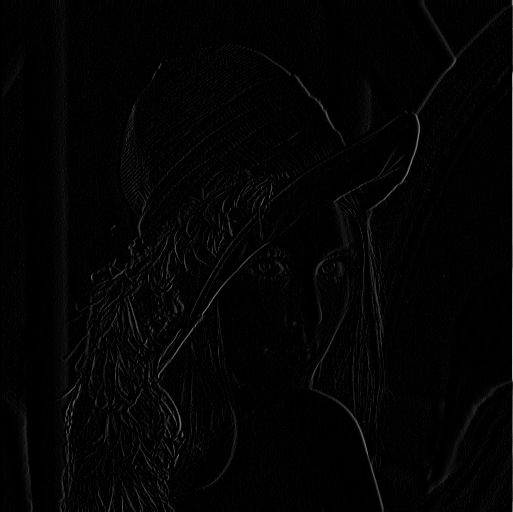
\includegraphics[width=0.45\linewidth]{discreteConvolution/lena_h3}
	}
	\caption{The Lena test image convolved with various kernels.}
	\label{fig:discreteConvolution.lena}
\end{figure}



\section{Fourier analyisis}

\section{Point operations}

\subsection{Image histogram}

\begin{figure}[ht]
\centering
	\subfigure[Original image]{
	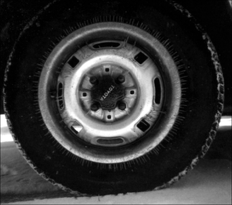
\includegraphics[width=0.45\linewidth]{pointOperations/tireBase}
	}
	\subfigure[Original image histogram]{
	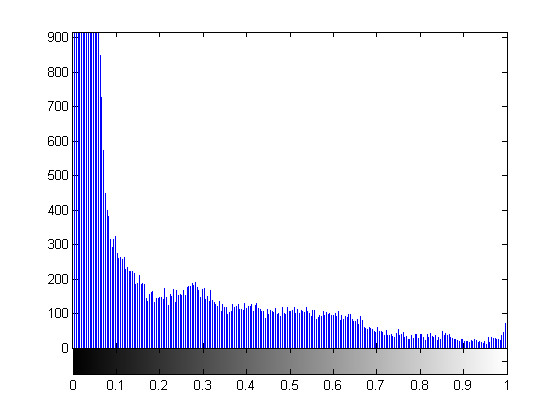
\includegraphics[width=0.45\linewidth]{pointOperations/tireBase_hist}
	}
\end{figure}

\subsection{Negative image histogram}

\begin{figure}[ht]
\centering
	\subfigure[Negative image]{
	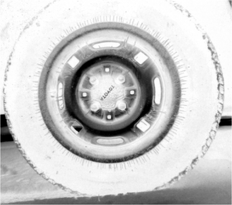
\includegraphics[width=0.45\linewidth]{pointOperations/tireNeg}
	}
	\subfigure[Negative image histogram]{
	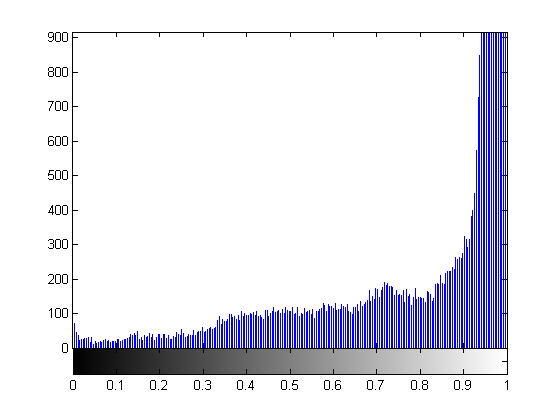
\includegraphics[width=0.45\linewidth]{pointOperations/tireNeg_hist}
	}
\end{figure}


\subsection{Power-law transformations}

\begin{figure}[ht]
\centering
	\subfigure[Gray-level expansion with $\gamma = 0.5$]{
	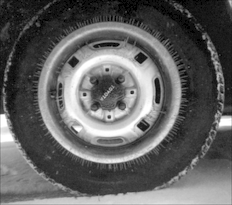
\includegraphics[width=0.45\linewidth]{pointOperations/tire_0_5}
	}
	\subfigure[Gray-level expansion histogram with $\gamma = 0.5$]{
	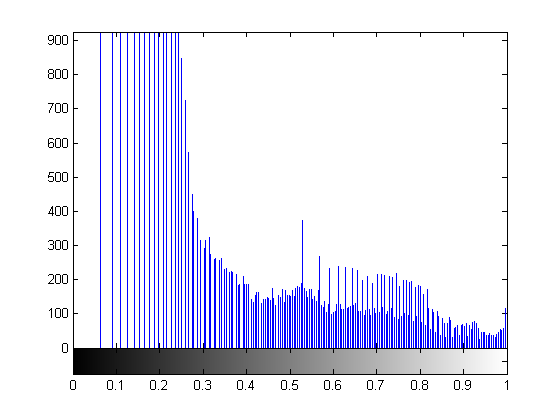
\includegraphics[width=0.45\linewidth]{pointOperations/tire_0_5_hist}
	}
	\subfigure[Gray-level compression with $\gamma = 1.3$]{
	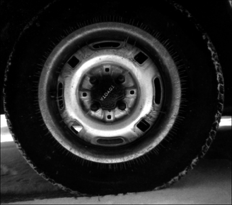
\includegraphics[width=0.45\linewidth]{pointOperations/tire_1_3}
	}
	\subfigure[Gray-level compression histogram with $\gamma = 1.3$]{
	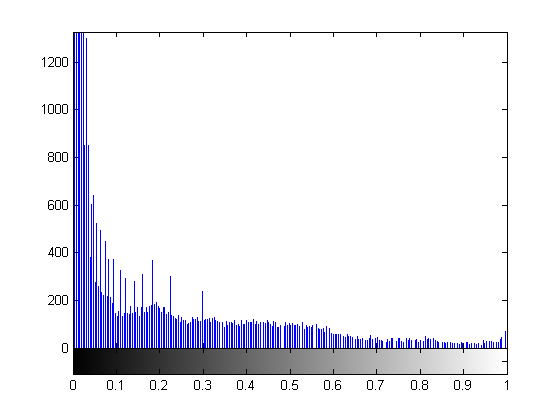
\includegraphics[width=0.45\linewidth]{pointOperations/tire_1_3_hist}
	}
\end{figure}


\subsection{Histogram equalization}


\begin{figure}[ht]
\centering
	\subfigure[Histogram equalized image]{
	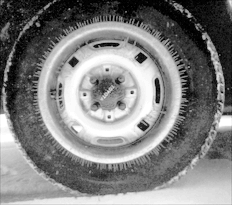
\includegraphics[width=0.45\linewidth]{pointOperations/tire_eq}
	}
	\subfigure[Histogram equalized image histogram]{
	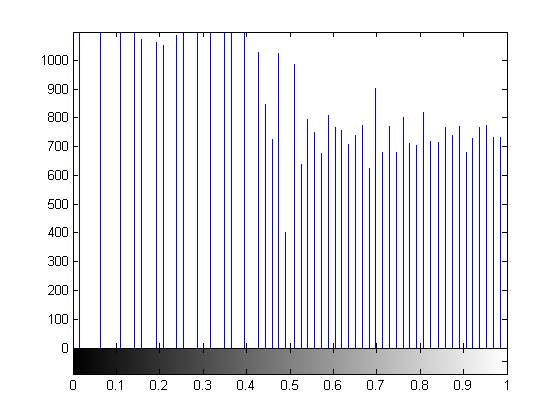
\includegraphics[width=0.45\linewidth]{pointOperations/tire_eq_hist}
	}
\end{figure}


\appendix
\newpage

\section{Matlab Code}
\subsection{PSNR}
\label{code-PSNR}
\lstinputlisting[language=Matlab]{"matlabFiles/PSNR.m"}


% -------- Bibliography --------
%\addcontentsline{toc}{chapter}{\hspace{13pt} References}
\bibliography{refs}

\end{document}  